\paragraph{comparison}

ComparisonGate is a gate for checking that one value is less than or equal to another. 
Compared numbers are divided into chunks, and chunk size and the number are configurable.

For a ComparisonGate with 8 4-bits chunks is like \figref{fig:comparison}.

\begin{figure}[!ht]
    \centering
    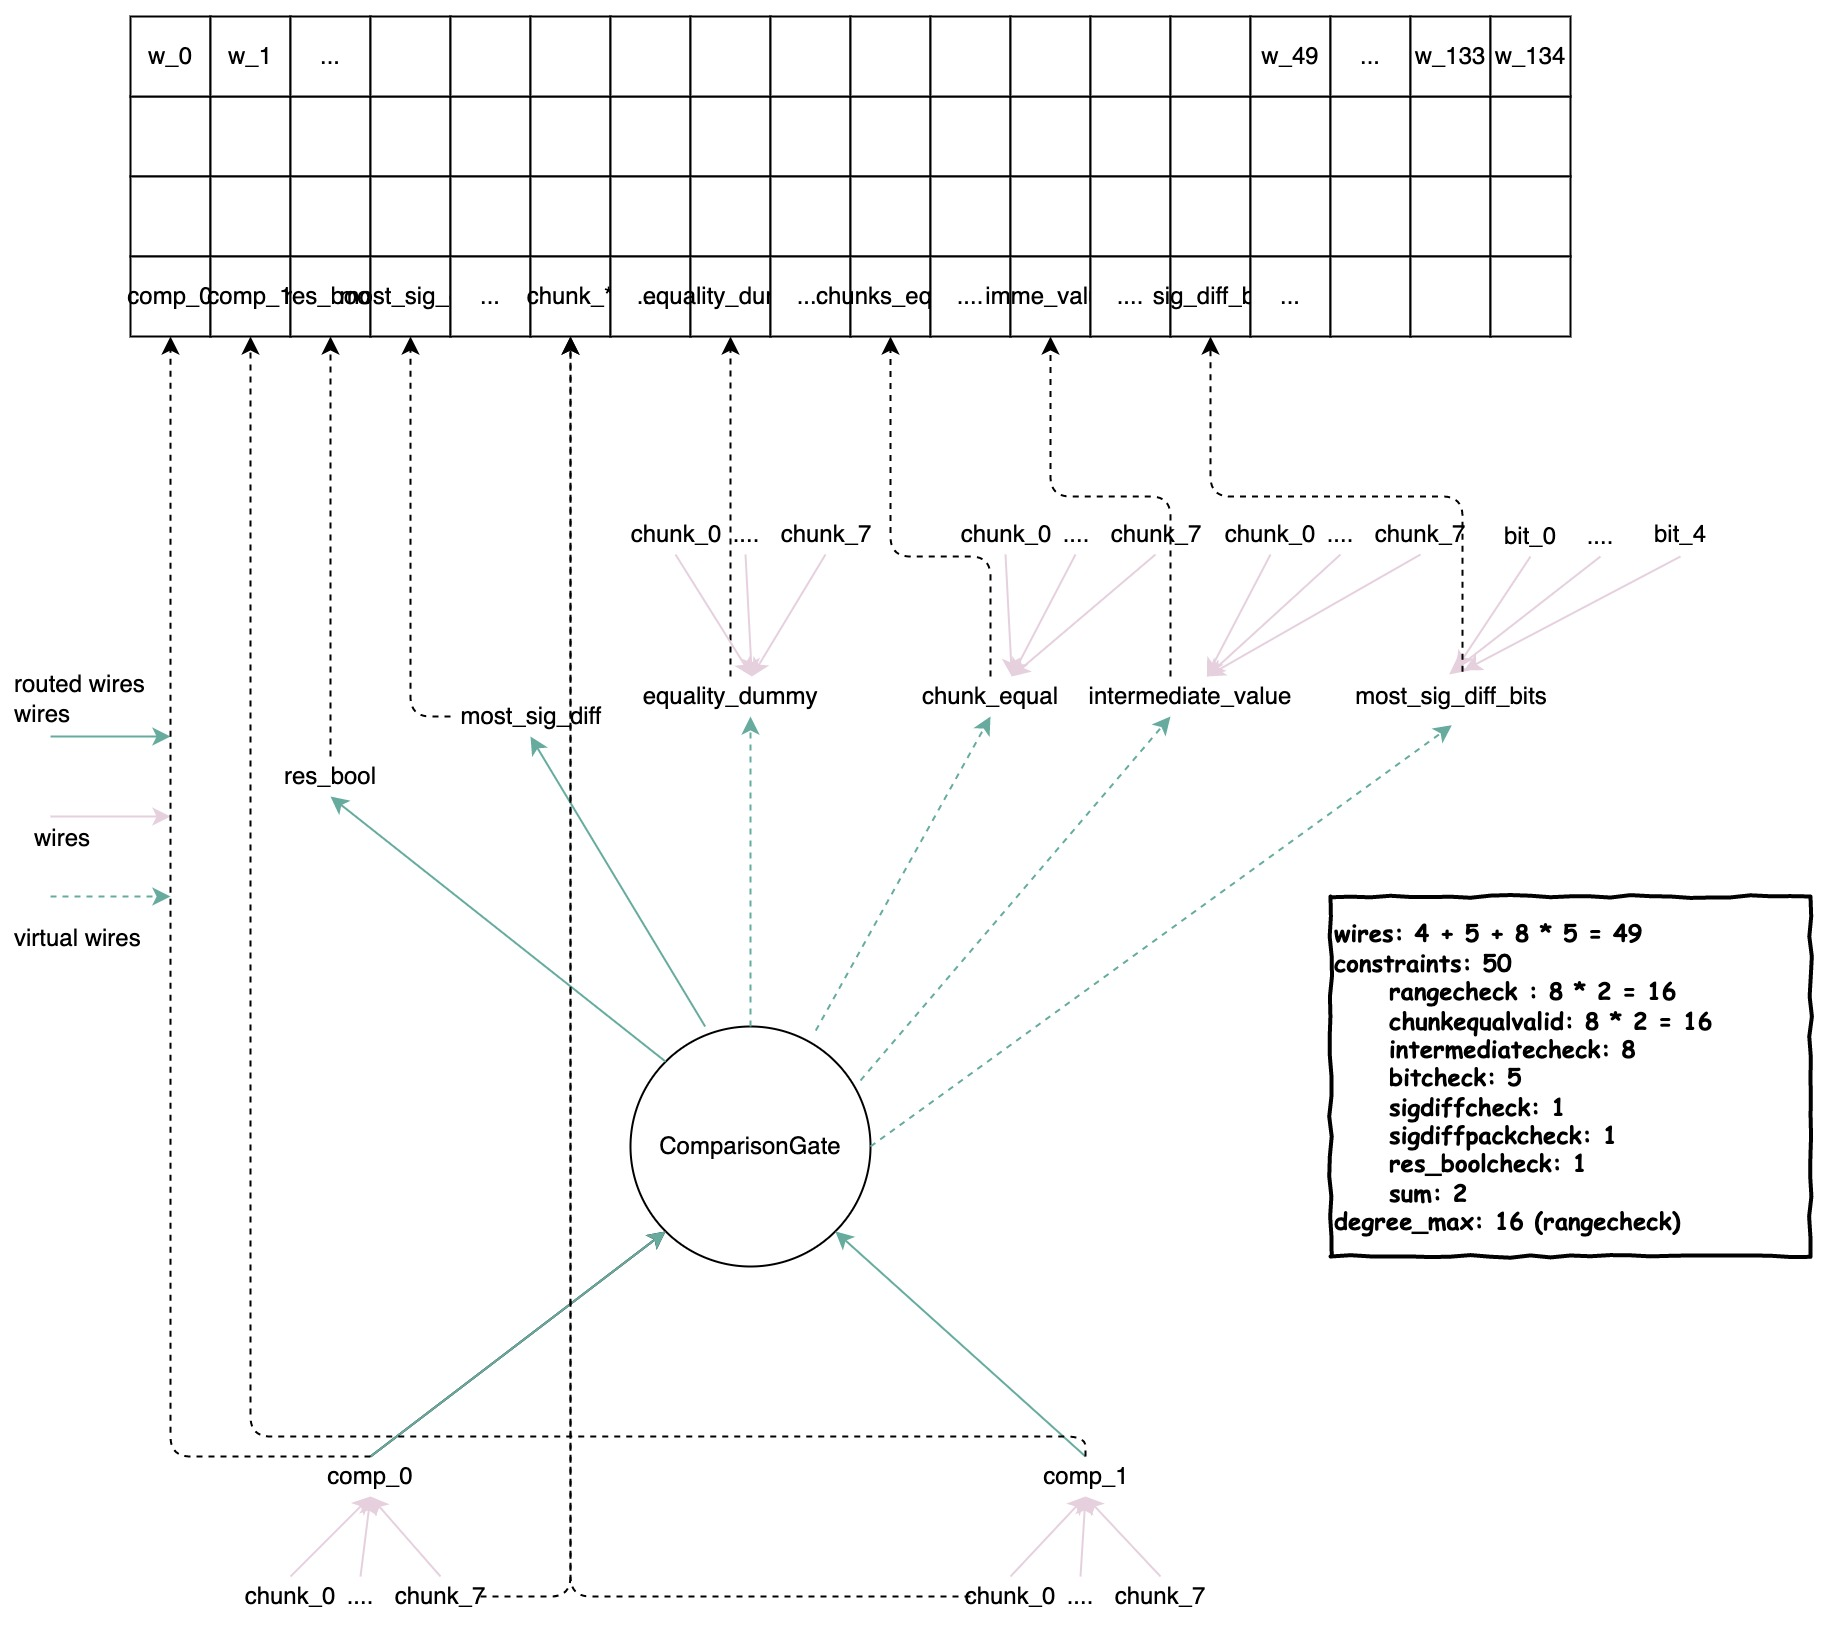
\includegraphics[width=0.6\textwidth]{gates/comparison.jpeg}
    \caption{ComparisonGate}
    \label{fig:comparison}
\end{figure}

The main idea of constraints:
\begin{itemize}
    \item Consistency of the sliced chunks and the original values.
    \item Range check for each chunk.
    \item If the chunks are equal, the difference is 0 and there is no inverse.
    \item Chunk by chunk so for most significant diff equals related intermediate\_value.
    \item If first <= second, the top \verb|n+1|-th bit of $(2^n + \text{most\_significant\_diff})$ will be 1.
\end{itemize}
